%Nama Kelompok: Hardware
%Kelas: D4 1B
%Alit Fajar 1174057
%Berlian 1174034
%Ichsan 1174058
%Kevin 1174059
%Iqbal Hambali 1174060


\section{Infrared Obstacle Detector}
	Sensor infrared obstacle detector memanfaatkan kondisi apabila infrared pada sensor ditutup maka LED notifikasi akan menyala,
sensor ini bekerja dengan memanfaatkan infrared, apabila cahaya infrared diterima dengan cahaya yang cukup terang maka lampu tidak menyala dan apabila 
cahaya infrared diterima dengan pencerahan cahaya yang kurang maka lampu akan menyala sebagai pengganti penerangan.

\subsection{Pengguunaan Infrared Obstacle Detector}
	Kegunaan dari Infrared Obstacle Detector digunakan untuk mendeteksi penerangan cahaya dengan memanfaatkan sinar infrared yang ada pada sensor tersebut.
 
\subsection{Cara Kerja Sensor}
	Cara kerja dari Infrared Obstacle Detector yaitu apabila ada penghalang yang menghalangi sinar infrared maka LED notifikasi akan menyala.

\subsection{Ilustrasi kerja sensor}

\ref{Keadaan lampu nyala
\begin{figure}[ht]
\centerline{\includegraphics[width=1\textwidth]{figures/nyala.JPG}}
\caption{Keadaan lampu nyala
\label{Keadaan lampu nyala
\end{figure}

\ref{Keadaan lampu mati}
\begin{figure}[ht]
\centerline{\includegraphics[width=1\textwidth]{figures/mati.JPG}
\caption{Keadaan lampu mati}
\label{Keadaan lampu mati}
\end{figure}

\subsection {Code}
Aplikasi penunjang yang kami gunakan dalam membuat code yang akan diterapkan di sensor kami adalah arduino, Berikut adalah code input yang digunkan dalam infrared sensor
\begin {verbatim}
void setup() {
pinMode(A0,INPUT);
pinMode(A1,OUTPUT);
pinMode(A2,OUTPUT);
pinMode(13,OUTPUT);
digitalWrite(A2,HIGH);
digitalWrite(A1,LOW);
Serial.begin(9600);
}

void loop() {
Serial.println(analogRead(A0));
delay(1000);
if(analogRead(A0) < 250){
digitalWrite(13,HIGH);
}
else{
digitalWrite(13,LOW);
}
}
\end{verbatim}

\section{Ambil Data InfraRed Obstacle Detector}

\subsection{Ambil Data}
	Ambil data dari uji coba Infrared Obstacle Detector dengan berbagai kertas bewarna, dari mulai delay 1000 sampai delay 100.
	
\subsection{Gambar Ambil Data}

\ref{Delay_1000}
\begin{figure}[ht]
\centerline{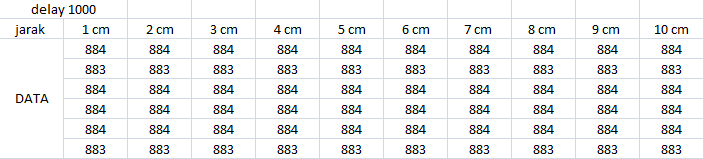
\includegraphics[width=1\textwidth]{figures/delay_1000}}
\caption{Hasil delay 1000}
\label{Hasil delay 1000}
\end{figure}

\ref{Delay_500}
\begin{figure}[ht]
\centerline{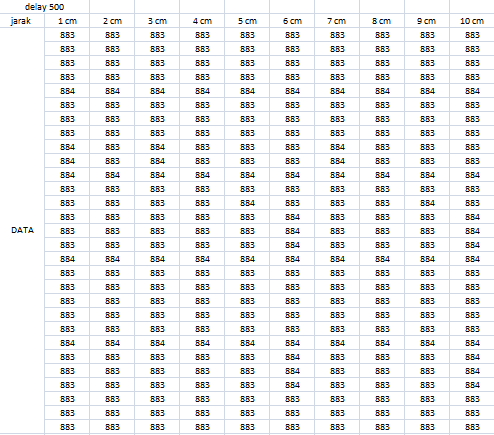
\includegraphics[width=1\textwidth]{figures/delay_500}}
\caption{Hasil delay 500}
\label{Hasil delay 500}
\end{figure}

\ref{Delay_100}
\begin{figure}[ht]
\centerline{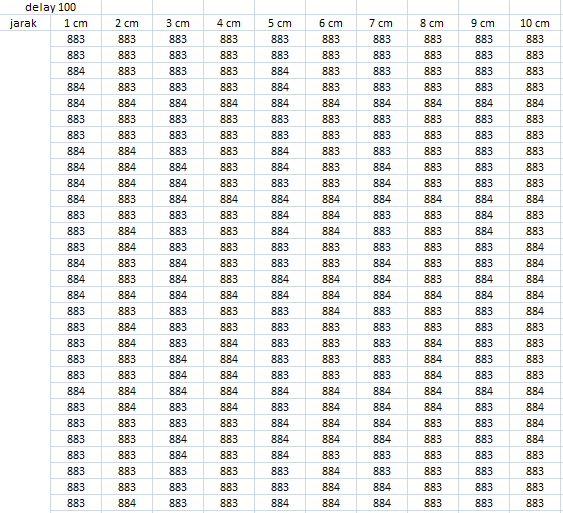
\includegraphics[width=1\textwidth]{figures/delay_100_1}}
\caption{Hasil delay 100}
\label{Hasil delay 100}
\end{figure}

\ref{Delay_100}
\begin{figure}[ht]
\centerline{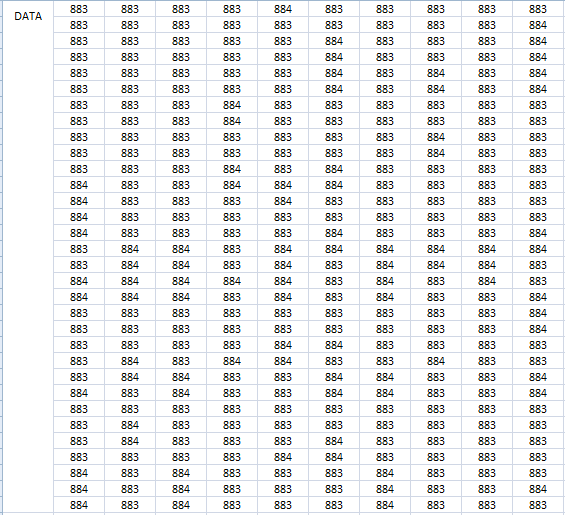
\includegraphics[width=1\textwidth]{figures/delay_100_2}}
\caption{Hasil delay 100}
\label{Hasil delay 100}
\end{figure}
